\section*{Exercises for Section~\ref{S:indexfamily}}
%
\begin{enumerate}
\item For each natural number $n$, let $A_n = \left\{n, n+1, n+2, n+3 \right\}$.  Use the roster method to specify each of the following sets: \label{exer:sec45-example1}

\begin{multicols}{2}
\begin{enumerate}
\yitem $\bigcap\limits_{j=1}^{3}A_j$
\item $\bigcup\limits_{j=1}^{3}A_j$
\item $\bigcap\limits_{j=3}^{7}A_j$
\yitem $\bigcup\limits_{j=3}^{7}A_j$
\item $A_9 \cap \left(\:\bigcup\limits_{j=3}^{7}A_j \right)$
\item $\bigcup\limits_{j=3}^{7}\left( A_9 \cap A_j \right)$
\end{enumerate}
\end{multicols}


\item For each natural number $n$, let 
$A_n = \left\{ k \in \N \left| \hspace{3pt} k \geq n \right. \right\}$.  Assuming the universal set is $\N$, use the roster method or set builder notation to specify each of the following sets: \label{exer:sec45-example2}

\begin{multicols}{2}
\begin{enumerate}
\yitem $\bigcap\limits_{j=1}^{5}A_j$
\item $\left(\: \bigcap\limits_{j=1}^{5}A_j \right)^c$
\yitem $\bigcap\limits_{j=1}^{5}A_j^c$
\yitem $\bigcup\limits_{j=1}^{5}A_j^c$
\item $\bigcup\limits_{j=1}^{5}A_j$
\yitem $\left(\: \bigcup\limits_{j=1}^{5}A_j \right)^c$
%\yitem $\bigcup\limits_{j=1}^{5}A_j^c$
%\yitem $\bigcap\limits_{j=1}^{5}A_j^c$
\item $\bigcap\limits_{j \in \N}^{}A_j$
\item $\bigcup\limits_{j \in \N}^{}A_j$
%\item $A_9 \cap \left( \bigcup\limits_{j=3}^{7}A_j \right)$
%\item $\bigcup\limits_{j=3}^{7}\left( A_9 \cap A_j \right)$
\end{enumerate}
\end{multicols}

\item For each positive real number $r$, define $T_r$ to be the closed interval 
$\left[ -r^2, r^2 \right]$. That is, 
\label{exer:indexpositivereals}% 
\[
T_r = \left\{ x \in \R \left| -r^2 \leq x \leq r^2 \right. \right\}\!.
\]
Let $\Lambda = \left\{ m \in \N \left| 1 \leq m \leq 10 \right. \right\}$.  Use either interval notation or set builder notation to specify each of the following sets:

\begin{multicols}{3}
\begin{enumerate}
\yitem $\bigcup\limits_{k \in \Lambda}^{}T_k$
\yitem $\bigcap\limits_{k \in \Lambda}^{}T_k$
\item $\bigcup\limits_{r \in \R^+}^{}T_r$
\item $\bigcap\limits_{r \in \R^+}^{}T_r$
\item $\bigcup\limits_{k \in \N}^{}T_k$
\item $\bigcap\limits_{k \in \N}^{}T_k$
\end{enumerate}
\end{multicols}

\item Prove Parts~(\ref{T:indexproperties2}) and~(\ref{T:indexproperties4}) of 
Theorem~\ref{T:indexproperties}.  Let $\Lambda$ be a nonempty indexing set and let 
$\mathscr{A} = \left\{ A_\alpha \mid \alpha \in \Lambda \right\}$ be an indexed family of sets. 
\label{exer:indexproperties}
\begin{enumerate}
\yitem For each $\beta \in \Lambda$, 
$A_\beta \subseteq \bigcup\limits_{\alpha \in \Lambda}^{}A_\alpha$.
\item $\left(\:\bigcup\limits_{\alpha \in \Lambda}^{}A_\alpha \right)^c = 
\bigcap\limits_{\alpha \in \Lambda}^{}A_{\alpha}^c$
\end{enumerate}

\item Prove Theorem~\ref{T:distributeindex}.  Let $\Lambda$ be a nonempty indexing set, let 
$\mathscr{A} = \left\{ A_\alpha \mid \alpha \in \Lambda \right\}$ be an indexed family of sets, and let $B$ be a set.  Then \label{exer:distributeindex}
\begin{enumerate}
\yitem $B \cap \left(\:\bigcup\limits_{\alpha \in \Lambda}^{}A_{\alpha} \right) 
= \bigcup\limits_{\alpha \in \Lambda}^{} \left( B \cap A_{\alpha} \right)$, and
\item $B \cup \left(\:\bigcap\limits_{\alpha \in \Lambda}^{}A_{\alpha} \right) 
= \bigcap\limits_{\alpha \in \Lambda}^{} \left( B \cup A_{\alpha} \right)$.
\end{enumerate}


\item Let $\Lambda$ and $\Gamma$ be nonempty indexing sets.  (\note The letter $\Gamma$ is the uppercase Greek letter gamma.) Also, let 
$\mathscr{A} = \left\{ A_\alpha \mid \alpha \in \Lambda \right\}$ and 
$\mathscr{B} = \left\{ B_\beta \mid \beta \in \Gamma \right\}$
be indexed families of sets.  Use the distributive laws in Exercise~(\ref{exer:distributeindex}) to: \label{exer:doubledistribute}
\begin{enumerate}
\item Write $\left(\: \bigcup\limits_{\alpha \in \Lambda}^{}A_\alpha\right) \cap \left(\: \bigcup\limits_{\beta \in \Gamma}^{}B_\beta \right)$ as a union of intersections of two sets.

\item Write $\left(\: \bigcap\limits_{\alpha \in \Lambda}^{}A_\alpha\right) \cup \left(\: \bigcap\limits_{\beta \in \Gamma}^{}B_\beta \right)$ as an intersection of unions of two sets.
\end{enumerate}




\item Let $\Lambda$ be a nonempty indexing set and let 
$\mathscr{A} = \left\{ A_\alpha \mid \alpha \in \Lambda \right\}$ be an indexed family of sets.  Also, assume that $\Gamma \subseteq \Lambda$ and $\Gamma \ne \emptyset$.    Prove that
\begin{multicols}{2}
\begin{enumerate}
\item $\bigcup\limits_{\alpha \in \Gamma}^{}A_\alpha \subseteq 
\bigcup\limits_{\alpha \in \Lambda}^{}A_\alpha$

\item $\bigcap\limits_{\alpha \in \Lambda}^{}A_\alpha \subseteq 
\bigcap\limits_{\alpha \in \Gamma}^{}A_\alpha$
\end{enumerate}
\end{multicols}



\item Let $\Lambda$ be a nonempty indexing set and let 
$\mathscr{A} = \left\{ A_\alpha \mid \alpha \in \Lambda \right\}$ be an indexed family of sets. 
\label{exer:indexsubsets}%

\begin{enumerate}
\yitem Prove that if $B$ is a set such that $B \subseteq A_\alpha$ for every 
$\alpha \in \Lambda$, then $B \subseteq \bigcap\limits_{\alpha \in \Lambda}^{}A_\alpha$.

\item Prove that if $C$ is a set such that $A_\alpha \subseteq C$ for every 
$\alpha \in \Lambda$, then $\bigcup\limits_{\alpha \in \Lambda}^{}A_\alpha \subseteq C$.
\end{enumerate}


\item For each natural number $n$, let \label{exer:pairwisedisjoint}
$A_n = \left\{ x \in \R \left| \hspace{3pt} n -1 < x < n \right. \right\}$.  Prove that 
$\left\{ A_n \left| \hspace{3pt} n \in \N \right. \right\}$ is a pairwise disjoint family of sets and that 
\linebreak
$\bigcup\limits_{n \in \N}^{}A_n = \left( \R^+ - \N \right)$.


\item For each natural number $n$, let 
$A_n = \left\{ k \in \N \left| \hspace{3pt} k \geq n \right. \right\}$.  
\label{exer:sec45-notpairdisjoint}
Determine if the following statements are true or false.  Justify each conclusion.

\begin{enumerate}
\item For all $j, k \in \N$, if $j \ne k$, then $A_j \cap A_k \ne \emptyset$.
\item $\bigcap\limits_{k \in \N}^{}A_k = \emptyset$
\end{enumerate}


\item Give an example of an indexed family of sets $\left\{ A_n \left| n \in \N \right. \right\}$ such all three of the following conditions are true: \label{exer:notpairdisjoint2}

\BeginTable
\BeginFormat
| p(6pt) | r | l |
\EndFormat
"  " (i) " For each $m \in \N$, $A_m \subseteq (0, 1)$; " \\
"  " (ii) " For each $j, k \in \N$, if $j \ne k$, then $A_j \cap A_k \ne \emptyset$; and " \\
"  " (iii) " $\bigcap\limits_{k \in \N}^{}A_k = \emptyset$. " \\
\EndTable


\item Let $\Lambda$ be a nonempty indexing set, let \label{exer:gendemorgan}
$\mathscr{A} = \left\{ A_\alpha \mid \alpha \in \Lambda \right\}$ be an indexed family of sets, and let $B$ be a set.  Use the results of Theorem~\ref{T:indexproperties} and 
Theorem~\ref{T:distributeindex} to prove each of the following:

\begin{enumerate}
\yitem $\left(\:\bigcup\limits_{\alpha \in \Lambda}^{}A_{\alpha} \right) - B 
= \bigcup\limits_{\alpha \in \Lambda}^{} \left( A_{\alpha} - B \right)$

\item $\left(\:\bigcap\limits_{\alpha \in \Lambda}^{}A_{\alpha} \right) - B 
= \bigcap\limits_{\alpha \in \Lambda}^{} \left( A_{\alpha} - B \right)$

\item $B - \left(\:\bigcup\limits_{\alpha \in \Lambda}^{}A_{\alpha} \right) 
= \bigcap\limits_{\alpha \in \Lambda}^{} \left( B - A_{\alpha} \right)$

\item $B - \left(\:\bigcap\limits_{\alpha \in \Lambda}^{}A_{\alpha} \right) 
= \bigcup\limits_{\alpha \in \Lambda}^{} \left( B - A_{\alpha} \right)$

\end{enumerate}
\end{enumerate}



\subsection*{Explorations and Activities}
\setcounter{oldenumi}{\theenumi}
\begin{enumerate} \setcounter{enumi}{\theoldenumi}
  \item \textbf{An Indexed Family of Subsets of the Cartesian Plane}.  \label{A:indexfamiliy}
Let $\R^*$ be the set of nonnegative real numbers, and for each $r \in \R^*$, let
\[
\begin{aligned}
C_r &= \left\{ (x, y) \in \R \times \R \mid x^2 + y^2 = r^2 \right\} \\
D_r &= \left\{ (x, y) \in \R \times \R \mid x^2 + y^2 \leq r^2 \right\} \\
T_r &= \left\{ (x, y) \in \R \times \R \mid x^2 + y^2 > r^2 \right\} = D_r^c. \\
\end{aligned}
\]
If $r > 0$, then the set $C_r$ is the circle of radius $r$ with center at the origin as shown in 
Figure~\ref{fig:activity-index}, and the set $D_r$ is the shaded disk (including the boundary) shown in Figure~\ref{fig:activity-index}.

\begin{figure}[h]
\begin{center}
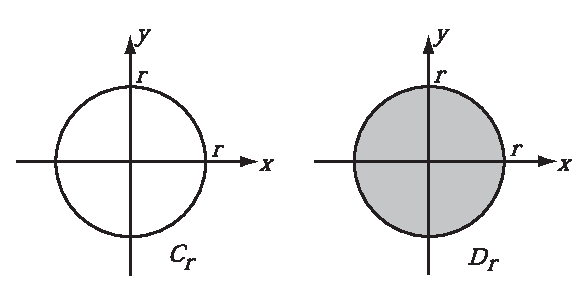
\includegraphics{figps-activitycircles.eps}
\end{center}
\caption{Two Sets for Activity~\ref{A:indexfamiliy}} \label{fig:activity-index}
\end{figure}

\begin{enumerate}
\item Determine $\bigcup\limits_{r \in \R^*}^{}C_r$ and $\bigcap\limits_{r \in \R^*}^{}C_r$.

\item Determine $\bigcup\limits_{r \in \R^*}^{}D_r$ and $\bigcap\limits_{r \in \R^*}^{}D_r$.

\item Determine $\bigcup\limits_{r \in \R^*}^{}T_r$ and $\bigcap\limits_{r \in \R^*}^{}T_r$.

\item Let $\mathscr{C} = \left\{ C_r \mid r \in \R^* \right\}$, 
$\mathscr{D} = \left\{ D_r \mid r \in \R^* \right\}$, and 
$\mathscr{T} = \left\{ T_r \mid r \in \R^* \right\}$.  Are any of these indexed families of sets pairwise disjoint?  Explain.
\end{enumerate}

\noindent
Now let $I$ be the closed interval $[0, 2]$ and let $J$ be the closed interval $[1, 2]$.
\begin{enumerate} \setcounter{enumii}{4}
\item Determine $\bigcup\limits_{r \in I}^{}C_r$, $\bigcap\limits_{r \in I}^{}C_r$, $\bigcup\limits_{r \in J}^{}C_r$, and $\bigcap\limits_{r \in J}^{}C_r$.

\item Determine $\bigcup\limits_{r \in I}^{}D_r$, $\bigcap\limits_{r \in I}^{}D_r$, $\bigcup\limits_{r \in J}^{}D_r$, and $\bigcap\limits_{r \in J}^{}D_r$.

\item Determine $\left(\: \bigcup\limits_{r \in I}^{}D_r \right)^c$, 
$\left(\: \bigcap\limits_{r \in I}^{}D_r \right)^c$, 
$\left(\: \bigcup\limits_{r \in J}^{}D_r \right)^c$, and 
$\left(\: \bigcap\limits_{r \in J}^{}D_r \right)^c$.
\label{A:indexfamily7}%


\item Determine $\bigcup\limits_{r \in I}^{}T_r$, $\bigcap\limits_{r \in I}^{}T_r$, $\bigcup\limits_{r \in J}^{}T_r$, and $\bigcap\limits_{r \in J}^{}T_r$.
\label{A:indexfamily8}%

\item Use De Morgan's Laws to explain the relationship between your answers in 
Parts~(\ref{A:indexfamily7}) and~(\ref{A:indexfamily8}).
\end{enumerate}
\end{enumerate}


\hbreak
\endinput
